% compile with
%   pdflatex --shel-escape p03-matrizes
% or
%   latexmk -pvc -pdf -latexoption=--shell-escape p03-matrizes
%

\documentclass[11pt,fleqn]{practice}

% Comente a linha seguinte para incluir as soluções
\tcbset{lowerbox=ignored}

\usetikzlibrary{calc}

\begin{document}

\institution{UFOP\quad DECOM}
\course{Programação de Computadores I}
\subtitle{Aula prática 3}
\title{Vetores, Matrizes e Gráficos}
\author{}
\date{2013--2}
\maketitle

\begin{abstract}
  Nesta aula você irá utilizar vetores para resolver diversos tipos de
  problemas. Para expressar a solução do problema, você poderá precisar
  usar operações escalares ou operações vetoriais.

  Você vai também aprender um pouco sobre como desenhar gráficos.
\end{abstract}

\tableofcontents

\section{Matrizes}

A estrutura fundamental de dados em Scilab é uma \textbf{matriz}. Uma
matriz é semelhante a uma \emph{tabela}, exceto que uma matriz pode ter
qualquer número de dimensões, enquanto uma tabela tem apenas duas
dimensões, que usualmente são chamadas de linhas e colunas. Por exemplo,
as matrizes $A$, $B$ e $C$, dadas a seguir, têm dimensões $1\times 5$,
$3\times 1$ e $3\times 2$, respectivamente:

\begin{align*}
  A &=
  \begin{bmatrix}
    3 & 5 & 7 & 12 & 9
  \end{bmatrix}
  &
  B &=
  \begin{bmatrix}
    8 \\
    5 \\
    7
  \end{bmatrix}
  &
  C &=
  \begin{bmatrix}
    3 & 8 \\
    12 & 5 \\
    9 & 7
  \end{bmatrix}  
\end{align*}

A matriz $A$, que tem apenas 1 linha, é também chamada de
\textbf{vetor-linha}, ou simplesmente \textbf{vetor}.  A matriz $B$, que
tem apenas 1 coluna, é também chamada de \textbf{vetor-coluna}.

Em Scilab, o valor denotado por uma variável é sempre uma matriz. Em
particular, um valor escalar, tal como $2$, $11.3$ ou \texttt{\%pi} é
visto como uma matriz de dimensão $1\times 1$.

\subsection{Criando matrizes}

\paragraph{Enumerando os elementos}

Os elementos são colocados entre colchetes. Elememtos de uma mesma linha
são separados por espaço ou vírgula (\texttt{,}), e as linhas são
separadas por ponto-e-vírgula (\texttt{;}).

Exemplo:
\begin{lst}{scilab}
-->A = [ 10, 20, 30, 40; 4, 3, 2, 1; 0.2, 4/10, 0.6, 1-0.8 ]
 A  =
 
    10.    20.    30.    40.  
    4.     3.     2.     1.   
    0.2    0.4    0.6    0.2
\end{lst}

\paragraph{Valores incrementados linearmente}

Os elementos de uma linha podem ser especificados por
\textbf{\texttt{$v_i$:$i$:$v_f$}}, que representa todos os valores de
$v_i$ até $v_f$, em incrementos de $i$.

Exemplos:
\begin{lst}{scilab}
-->E = [ 0 : 2 : 8 ]
 E  =
 
    0.    2.    4.    6.    8.  
 
-->F = [ 3 : 0.3 : 2*2+1 ]
 F  =
 
    3.    3.3    3.6    3.9    4.2    4.5    4.8  
 
-->G = [ -2:2:4 ; 1:-3:-8 ]
 G  =
 
  - 2.    0.    2.    4.  
    1.  - 2.  - 5.  - 8.  
\end{lst}

\paragraph{Matrizes especiais}

A função \textbf{\texttt{zeros}} cria uma matriz de zeros. A função
\textbf{\texttt{ones}} cria uma matriz de uns. A função
\textbf{\texttt{eye}} cria uma matriz diagonal. As dimensões são
especificadas pelos arguemntos da função.

Exemplos:
\begin{lst}{scilab}
-->Z = zeros(2, 3)    // matriz 2x3 de zeros
 Z  =
 
    0.    0.    0.  
    0.    0.    0.  
 
-->O = ones(2, 3)    // matriz 2x3 de uns
 O  =
 
    1.    1.    1.  
    1.    1.    1.  
 
-->D = eye(3, 4)    // matriz diagonal 3x4
 D  =
 
    1.    0.    0.    0.  
    0.    1.    0.    0.  
    0.    0.    1.    0.
\end{lst}

\paragraph{Criando matrizes a partir de sub-matrizes}

Uma matriz podem ser usada para criar uma outra matriz.

Exemplos:
\begin{lst}{scilab}
-->A = [0:2:6]
 A  =
 
    0.    2.    4.    6.  
 
-->B = [A; 1:4]
 B  =
 
    0.    2.    4.    6.  
    1.    2.    3.    4.
\end{lst}


\subsection{Operações com matrizes}

\paragraph{Aplicação de funções a matrizes}

Funções usuais sobre números, como, por exemplo, as funções
\texttt{abs}, \texttt{sqrt}, \texttt{log}, \texttt{sin} e \texttt{cos},
também podem ser aplicadas a matrizes de valores numéricos. Nesse caso,
elas operam sobre cada um dos elementos da matriz, de maneira
independente.

Exemplo:
\begin{lst}{scilab}
-->X = [0, %pi/2, %pi, 3*%pi/2, 2*%pi]
 X  =
 
    0.    1.5707963    3.1415927    4.712389    6.2831853  
 
-->Y = sin(X)
 Y  =
 
    0.    1.    1.225D-16  - 1.  - 2.449D-16  
\end{lst}

\paragraph{Transposição}

O opeador pós-fixo \texttt{'} calcula a transposta de uma matriz.

Exemplo:
\begin{lst}{scilab}
-->A = [ 1 8 9 5; 2 3 4 0 ]
 A  =
 
    1.    8.    9.    5.  
    2.    3.    4.    0.  
 
-->A'
 ans  =
 
    1.    2.  
    8.    3.  
    9.    4.  
    5.    0.
\end{lst}


\paragraph{Operações entre matrizes e escalares}

Os operadores aritméticos abaixo podem ser usados para realizar uma
operação aritmética entre um escalar $k$ e cada elemento de uma matriz
$A$.

Nos exemplos apresentados na tabela, considere que \texttt{M} é a matriz
\texttt{[2, 4, 6; 5, 3, 1]}:

\begin{center}
  \begin{tabular}{p{2cm}lp{9cm}} \hline
    \textbf{operação} & \textbf{descrição} & \textbf{exemplo} \\\hline
    \texttt{$k$ + $A$}\newline \texttt{$A$ + $k$}  & adição & \texttt{M + 2 = [4, 6, 8; 7, 3, 1]} \\\hline
    \texttt{$k$ - $A$}\newline \texttt{$A$ - $k$}  & subtração & \texttt{M - 1 = [1, 3, 5 ;4, 2, 0]} \\\hline
    \texttt{$k$ * $A$}\newline \texttt{$A$ * $k$}  & multiplicação & \texttt{M * 2 = [4, 6, 8; 7, 3, 1]} \\\hline
    \texttt{$A$ / $k$}\newline \texttt{$k$ ./ $A$}  & divisão & \texttt{M / 2 = [1, 2 ,3; 2.5, 1.5, 0.5]}\newline  \texttt{2 ./ M = [1., 0.5, 0.333; 0.4, 0..6666, 2.]} \\\hline
    \texttt{$k$ .\textasciicircum $A$}\newline \texttt{$A$ .\textasciicircum\ $k$}  & potenciação & \texttt{M .\textasciicircum 2 = [4, ,16, 36; 25, 9, 1]}\newline \texttt{2 .\textasciicircum M = [4, ,16, 64; 32, 8, 2]} \\\hline
  \end{tabular}
\end{center}

Exemplo:
\begin{lst}{scilab}
-->m = [3:6; 3:-1:0]
 m  =
 
    3.    4.    5.    6.  
    3.    2.    1.    0.  
 
-->(m.^2 - 1) / 2
 ans  =
 
    4.    7.5    12.    17.5  
    4.    1.5    0.   - 0.5
\end{lst}

\paragraph{Operações matriciais elemento a elemento}

Os operadores aritméticos abaixo podem ser usados para realizar uma
operação aritmética entre duas matrizes $A$ e $B$ de mesma dimensão,
\emph{elemento a elemento}.

Nos exemplos apresentados na tabela, considere que \texttt{M} e
\texttt{N} são as seguintes matrizes: \texttt{M=[2, 4, 6; 5, 3, 1]} e
\texttt{N=[1, 2, 3; 4, 5, 6]}

\begin{center}
  \begin{tabular}{llp{9cm}} \hline
    \textbf{operação} & \textbf{descrição} & \textbf{exemplo}\\\hline
    \texttt{$A$ + $B$} & adição & \texttt{M + N = [3, 6, 9; 9, 8, 7]}\\\hline
    \texttt{$A$ - $B$} & subtração & \texttt{M - N = [1, 2, 3; 1, -2, -5]} \\\hline
    \texttt{$A$ .* $B$} & multiplicação & \texttt{M .* N = [2, 8, 18; 20, 15, 6]}\\\hline
    \texttt{$A$ ./ $B$} & divisão & \texttt{M ./ N = [2., 2., 2.; 1.25, 0.6, 0.1666]}\\\hline
    \texttt{$A$ .\textasciicircum\ $B$} & potenciação & \texttt{M \textasciicircum\ N = [2, 16, 729; 1024, 125, 6]} \\\hline
  \end{tabular}
\end{center}

Exemplo:
\begin{lst}{scilab}
-->A = [3:6; 3:-1:0]
 A  =
 
    3.    4.    5.    6.  
    3.    2.    1.    0.  
 
-->B = [0:3; 1 5 2 0]
 B  =
 
    0.    1.    2.    3.  
    1.    5.    2.    0.  

-->C = 2*eye(2, 4)
 C  =
 
    2.    0.    0.    0.  
    0.    2.    0.    0.  
  
-->A .^ B + A .* C
 ans  =
 
    7.    4.     25.    216.  
    3.    36.    1.     1.    
\end{lst}

\paragraph{Operações matriciais}

Além da adição (\texttt{$A$ +$B$}) e da subtração (\texttt{$A$ -$B$}), descritas anteriormente, estão também definidos outros operadores matriciais, relacionados na tabela a seguir. Nas operações \texttt{$A$ * $B$} e \texttt{$A$ / $B$}, as matrizes $A$ e $B$ devem ser de dimensõee ($n\times k$)  e ($k \times n$), respecitvamente. Na operação \texttt{$A$ \textasciicircum\ $k$}, onde $k$ é um escalar, a matriz $A$ deve ser uma matriz quadrada, isto é, de dimensão ($n \times n$), e  \texttt{$A$ \textasciicircum\ $k$} é o mesmo que \texttt{$A$ * $A$ * \ldots * $A$}.\footnote{Não confundir esta operação com a operação  \texttt{$A$ .\textasciicircum\ $k$}, que significa elevar cada um dos elemento de $A$ a $k$}. Nos exemplos da tabela a seguir, considere que \texttt{M=[4 5; 5 4]} e \texttt{N=[1, 2; 3, 4]}.
\begin{center}
  \begin{tabular}{llp{9cm}} \hline
    \textbf{operação} & \textbf{descrição} & \textbf{exemplo}\\\hline
     \texttt{$A$ * $B$} & multiplicação & \texttt{M * N = [14, 13; 32, 31 ]} \\\hline
    \texttt{$A$ / $B$} & divisão & \texttt{M * N = [-0.5, 1.5; -4, 3]} \\\hline
    \texttt{$A$ \textasciicircum\ $k$} & exponenciação & \texttt{M \textasciicircum\ 6 = [7, 10; 15, 22 ]}  \\\hline
  \end{tabular}
\end{center}

Exemplo:
\begin{lst}{scilab}
-->A = [ 1 , 2; 3, 4 ]
 A  =
 
    1.    2.  
    3.    4.  
 
-->B = [2, 2; 1, 0]
 B  =
 
    2.    2.  
    1.    0.  
 
-->C = A * B
 C  =
 
    4.     2.  
    10.    6.  
 
-->D = A ^ 2  // D = A * A
 D  =
 
    7.     10.
    15.    22.
 
-->E = B^-1   // E = inversa de B
 E  =
 
    0.     1. 
    0.5  - 1.
 
-->B * B^-1   // o produto de uma mat. pela sua inversa é a mat. identidade
 ans  =
 
    1.    0.  
    0.    1.  
\end{lst}

\paragraph{Algumas funções úteis sobre matrizes}

\begin{center}
  \begin{tabular}{ll} \hline
    \textbf{função} & \textbf{descrição} \\\hline
    \texttt{$n$ = length($A$)} & número de elementos da $A$ \\\hline
    \texttt{[$l$,$c$] = size($A$)} & número de linhas e colunas de $A$ \\\hline
    \texttt{$s$ = sum($A$)} & soma dos elementos de $A$ \\\hline
    \texttt{$s$ = prod($A$)} & produto dos elementos de $A$ \\\hline
    \texttt{$s$ = mean($A$)} & média dos elementos de $A$ \\\hline
  \end{tabular}
\end{center}

Exemplo:
\begin{lst}{scilab}
-->A = [ 1 8 9 5; 2 3 4 0 ]
 A  =
 
    1.    8.    9.    5.  
    2.    3.    4.    0.  
 
-->[linhas,colunas] = size(A)
 colunas  =
 
    4.  
 linhas  =
 
    2.  

-->sum(A)
 ans  =

    32.
\end{lst}


\section{Desenhando Gráficos}

Para desenhar um gráfico de uma maneira simples, siga os passos
seguintes:

\begin{enumerate}
  \item É bom limpar a janela de gráficos (também chamada janela de
  figuras) antes de começar a construir um novo desenho. Para tanto use
  o comando \texttt{clf}.

  \item Defina um vetor\footnote{Vetores são matrizes
    unidimensionais. Um vetor linha é uma matriz contendo somente uma
    linha. Um vetor coluna é uma matriz contendo somente uma coluna.}
  contendo as abscissas dos pontos a serem plotados. A notação de
  progressão aritmética pode ser usada, indicando o limite inferior, a
  razão, e o limite superior.

   Exemplo:
   \begin{lst}{scilab}
// vetor linha formado pelas abscissas dos pontos a serem plotados
x = [-%pi : 0.2 : %pi];
   \end{lst}

   \item Calcule o vetor de valores das ordenadas dos pontos a serem
   plotados. Pode-se usar operações aritméticas ou funções com vetores
   para construir este vetor a partir do vetor das abscissas.

   Exemplo:
   \begin{lst}{scilab}
// vetor linha formado pela aplicação da função
// f(x) = x * sin(x) - x^3 / (2*pi)
// a cada elemento do vetor das abscissas
y = x .* sin(x) - x .^ 3 / (2*%pi);
   \end{lst}

   \item Para desenhar o gráfico, use a função \texttt{plot}, passando o
   vetor das abscissas e o vetor das ordenadas como argumentos. Pode-se
   desenhar vários gráficos ao mesmo tempo. Para cada gráfico use dois
   vetores (abscissas e ordenadas).

   A função \texttt{title} permite dar um título ao desenho.

   As funções \texttt{xlabel} e \texttt{ylabel} podem ser usadas para
   rotular os eixos do desenho.

   A função \texttt{legend} coloca legendas nos gráficos desenhados.

   A expressão \texttt{set(gca(), "grid", [1 1])} desenha uma grade.

   Exemplo:
   \begin{lst}{scilab}
// desenha o gráfico
plot(x, y);
title("Gráfico de funções");
xlabel("x");
ylabel("y");
legend("Resultado");
set(gca(), "grid", [1 1]);
   \end{lst}
   A seguir temos o desenho produzido por este exemplo.
   \begin{center}
     \includegraphics[width=\linewidth]{images/grafico}
   \end{center}
\end{enumerate}

\textbf{Observação}: O comando \texttt{figure} pode ser usado para
alocar janelas distintas para gráficos desenhados em programas. Por
exemplo, você poderá desenhar os dois gráficos, cada um em uma janela,
do seguinte modo:

\begin{lst}{scilab}
figure(1);
// inclua aqui os comandos para plotar o gráfico da janela 1
figure(2);
// inclua aqui os comandos para plotar o gráfico da janela 2
\end{lst}

\pagebreak

\begin{task}[breakable]{Posição e velocidade de uma bola \numex{2.10}}{}
  Se uma bola estacionária é lançada da altura $h_0$ acima da superfície
  da Terra, com velocidade vertical $v_0$, a posição e a velocidade da
  bola como função do tempo serão dadas pelas equações
  \[ h(t) = \frac{1}{2}gt^2 + v_0t + h_0 \]
  \[ v(t) = gt + v_0 \] onde $g$ é a aceleração da gravidade
  ($-9,8m/s^2$), $h$ é a altura acima da superfície da Terra (assumindo
  ausência de atrito do ar) e $v$ é a componente vertical da velocidade.

  Escreva um programa que solicite ao usuário a altura inicial da bola
  em $m$ e a velocidade de lançamento da bola em $m/s$, depois desenhe a
  altura e velocidade em função do tempo. Não deixe de incluir as
  legendas apropriadas no seu desenho.

  \begin{runexample}
Lançamento de uma bola
----------------------
altura inicial da bola (m): 20
velocidade de lançamento da bola (m/s): 46
  \end{runexample}
  \begin{center}
    \includegraphics[width=.8\linewidth]{images/bola}
  \end{center}

  \tcblower
  \solution
  \lstinput{scilab}{listings/p03/bola.sce}
\end{task}

\pagebreak

\section{Operações usando matrizes}

\begin{task}[breakable]{Objeto movendo-se em trajetória circular \numex{2.20}}{}
  Um objeto movendo-se em trajetória circular é apresentado na figura a
  seguir, onde $r$ é o raio da trajetória (em m), $v$ é a velocidade
  tangencial do objeto (em m/s), e $a$ é a sua aceleração centrípeta (em
  $\text{m}/\text{s}^2$), dada pela equação $ a = v^2/r $

  \begin{center}
    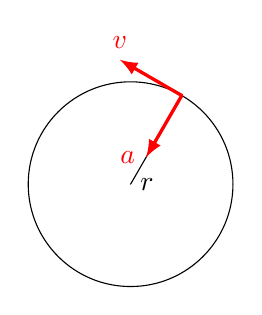
\begin{tikzpicture}[scale=1.3,cap=round,>=latex]
      % Draw Circle radius 1 cm
      \draw (0,0) circle (1cm);
      % radius vector at angle 60
      \draw [name=radius] (0,0)  node[right] {$r$}  -- (60:1cm);
      % the velocity vector
      \draw [name=velocity,very thick,->, red] (60:1cm) --  ($(60:1cm)!0.7cm!-90:(0,0)$) node[above] {$v$};
      % acceleration vector directed inward
      \draw [name=acceleration,very thick,->,red] (60:1cm) --  (60:0.3cm) node [left] {$a$} ;
    \end{tikzpicture}
    % \caption{Trajetória circular.}
    % \label{fig:circ-orbit}
  \end{center} 

  Considere que a aceleração gravitacional é $g = 9,81 \text{ m/s}$ e
  que a velocidade do som -- ou 1 Mach -- é 340 m/s.  Escreva um
  programa Scilab para traçar os gráficos mostrados abaixo, relativos à
  trajetória circular de uma aeronave:

  \begin{enumerate}
    \item Desenhe o gráfico da velocidade versus raio da trajetória,
    para valores de velocidade variando de 0,5 a 2,0 Mach, em intervalos
    de 0,1 Mach, supondo que a aceleração $a$ permanece com o valor
    constante 2$g$.
    \item Desenhe, na mesma janela, o gráfico de velocidade
    versus raio da trajetória, para a mesma faixa de valores de
    velocidade tangencial, supondo que a aceleração é 7$g$.
    \item Desenhe, em uma outra janela, o gráfico de raio versus
    aceleração centrípeta, para valores da aceleração de 2$g$ a 8$g$, em
    intervalos de 1$g$, supondo uma velocidade tangencial de 0,85 Mach.
  \end{enumerate}

  \begin{center}
    \includegraphics[width=.6\linewidth]{images/trajetoria-circular-rxv}\\
    \includegraphics[width=.6\linewidth]{images/trajetoria-circular-rxa}
  \end{center}

  \tcblower
  \solution
  \lstinput{scilab}{listings/p03/chapmann-2-20.sce}
\end{task}

\pagebreak 

\section{Usando vetores e operações vetoriais}

\begin{task}[breakable]{Série de Taylor}{}
  O logaritmo natural de um número real $z$, tal que $0 < z < 2$, pode
  ser aproximado pela série de Taylor a seguir:
  \[ \ln{(z)} = (z-1) - \frac{(z-1)^2}{2} + \frac{(z-1)^3}{3} -
  \frac{(z-1)^4}{4} + \cdots \]

  Em uma aproximação por série, quanto maior o número de termos
  considerados, mais próximo o valor do somatório estará do valor de
  $\ln{(z)}$.

  Faça um programa Scilab para calcular e imprimir o valor aproximado do
  logaritmo de um número real $z$ ($0< z< 2$), dado pela série de
  Taylor. O programa deve solicitar ao usuário o valor de $z$ e o número
  $n$ de termos da série a serem usados no cálculo do logaritmo natural
  de $z$.
  \\[1em]
  \textbf{\emph{Dicas\/}}:\newline
  Encontre o \textbf{termo geral} da série: $t_i$ (o $i$-ésimo termo).

  Como $t_i$ pode ser obtido a partir de $i$?

  Observe que cada termo é uma fração:
  \begin{itemize}
    \item o numerador da fração é uma potência com base $z-1$ e expoente
    $i$.
    \item o denominador da fração é $i$.
    \item o sinal dos termos alternam entre $+1$ e $-1$. Este sinal pode
    ser obtido facilmente usando uma potência de $-1$. Lembre-se que
    $-1$ elevado a um expoente par sempre resulta em $+1$. Já se o
    expoente for ímpar o resultado será $-1$.
  \end{itemize}
  Logo o termo geral da série é
  \[ t_i = (-1)^{i-1} \times \frac{(z-1)^i}{i} \]
  a partir do qual pode-se obter os termos individuais:
  \[ t_1 = (-1)^{1-1} \times \frac{(z-1)^1}{1} = (-1)^0 \times \frac{(z-1)^1}{1} = 1 \times \frac{z-1}{1} = z - 1 \]
  \[ t_2 = (-1)^{2-1} \times \frac{(z-1)^2}{2} = (-1)^1 \times \frac{(z-1)^2}{2} = -1 \times \frac{(z-1)^2}{2} = - \frac{(z-1)^2}{2} \]
  \[ t_3 = (-1)^{3-1} \times \frac{(z-1)^3}{3} = (-1)^2 \times \frac{(z-1)^3}{3} = 1 \times \frac{(z-1)^3}{3} = \frac{(z-1)^3}{3} \]
  \[ t_4 = (-1)^{4-1} \times \frac{(z-1)^4}{4} = (-1)^3 \times \frac{(z-1)^4}{4} = -1 \times \frac{(z-1)^4}{4} = - \frac{(z-1)^4}{4} \]
  \[ \vdots \]

  Uma vez conhecido a equação do termo geral da série:
  \begin{enumerate}
    \item Crie um vetor com valores de 1 a $n$ (os índices dos termos da
    série).
    \item Calcule os termos da série usando operações escalares e
    vetoriais sobre o vetor dos índices.
    \item A função \texttt{sum} pode ser usada para calcular a soma de
    todos elementos de uma matriz. Por exemplo, \texttt{sum([2,6,4,8])}
    produz como resultado o valor \texttt{20}. Use a função \texttt{sum}
    para somar os termos da série.
    \item Compare o resultado dado pelo seu programa com o valor
    calculado por meio da função \texttt{log} predefinida em Scilab.
  \end{enumerate}

  \begin{runexample}
Cálculo aproximado do logaritmo de z (0<z<2) 
--------------------------------------------
Digite um número no intervalo (0-2): 1.3
Digite o número de termos para o cálculo: 8

Valor aproximado do logaritmo de 1.3 = 0.262363
Usando a função predefinida = 0.262364
  \end{runexample}

  \tcblower
  \solution
  \lstinput{scilab}{listings/p03/p03-taylor.sce}
\end{task}

\end{document}
